% \documentclass{ctexart}
% Other classes are available too:
\documentclass{ctexrep}
% \documentclass{ctexbook}
% \documentclass{ctexbeamer}

%% You can change the font if necessary.
% \setCJKmainfont{BabelStone Han}
% \setCJKsansfont{Noto Sans CJK SC}
%---------------------这里添加所需的package--------------------------------
\usepackage{url}
\usepackage{amsmath}
\usepackage{graphicx}
\usepackage{hyperref}
\usepackage{varwidth}
\usepackage{lipsum}% for context
\usepackage[demo]{graphicx}
\usepackage{caption}
\usepackage{subcaption}
\newenvironment{pcenter}
 {\begin{center}\begin{varwidth}{\textwidth}\raggedright}
 {\end{varwidth}\end{center}}
%--------------------------------------------------------------------------
\makeatletter
\def\BState{\State\hskip-\ALG@thistlm}
\makeatother
\begin{document}
%-----------------------------------------------------------------------------

% \title{标题} % 报告主题
% \author{姓名} % 学生姓名
% \Csupervisor{袁烨} % 指导教师姓名
% \CstudentNum{UXXXXX} % 学号
% \Cmajor{XXXXXX} % 专业名称
% \Cschoolname{人工智能与自动化学院} % 学院名
% \date{XXXX年XX月XX日} % 日期

\title{ 
\huge \textsc{华中科技大学}\\
        \Large \textsc{数据科学基础大作业}
		\\ [2.0cm]
% 		\HRule{0.5pt} \\
		\LARGE \textbf{\uppercase{矩阵分解}}
% 		\HRule{2pt} \\ [0.5cm]
		\normalsize  \vspace*{5\baselineskip}
}


\author{
\begin{pcenter}
院\:\: \:\:系:人工智能与自动化学院\\ 
专业班级:自实1801\\
学生姓名:李子怡\\
学生学号:U201814168\\
指导教师:袁烨

\end{pcenter}
}


\date{2021年5月15日}

\maketitle

%-----------------------------------------------------------------------------

\pdfbookmark[0]{封面}{title}         % 封面页加到 pdf 书签
\maketitle
\frontmatter
\pagenumbering{Roman}              % 正文之前的页码用大写罗马字母编号.正文之前的页码隐藏,无需显示
%-----------------------------------------------------------------------------
%==========================把目录加入到书签==============================%%%%%%

\tableofcontents
\thispagestyle{empty}				%不显示罗马数字
\addtocontents{toc}{\protect\thispagestyle{empty}}


\mainmatter %% 以下是正文
%%%%%%%%%%%%%%%%%%%%%%%%%%%--------main matter-------%%%%%%%%%%%%%%%%%%%%%%%%%%%%%%%%%%%%
\pagestyle{plain}%plain
%\cfoot{\thepage{\zihao{5}\bf\usefonttimes}}
%\renewcommand{\baselinestretch}{1.6}
%\setlength{\baselineskip}{23pt}
\baselineskip=23pt  % 正文行距为 23 磅
\pagenumbering{arabic}
%此处书写正文-------------------------------------------------------------------------------------
\chapter{摘要}
本报告主要针对矩阵分解这一数学方法进行分析,首先在 \autoref{chap:history} 探索矩阵分解的历史发展,与目前的瓶颈与未来的发展方向。其次在\autoref{chap:method}主要且基础的分解算法LU分解、QR分解与SVD分解进行了具体算法步骤的推导与分析。最重要的是\autoref{chap:application}中,对不同的方法进行不同的应用,并进行分析与优化,主要为:LU分解用于求解线性方程组,QR分解用于求取矩阵的特征根和SVD分解用于图像压缩与推荐系统。






\chapter{矩阵分解}
\label{chap:history}
\section{分解方法发展与概要}
矩阵分解已经有了悠久的历史。\cite{matrix_jiqi}

在数值分析和线性代数中,lower–upper (LU) decomposition分解或因子分解将矩阵作为下三角矩阵和上三角矩阵的乘积。有时也包括置换矩阵。 LU分解可以被视为高斯消元的矩阵形式。 计算机通常使用LU分解来求解线性方程的平方系统,并且当反转矩阵或计算矩阵的行列式时,它也是关键步骤。 LU分解由数学家Tadeusz Banachiewicz于1938年引入。

Cholesky分解或Cholesky分解是将Hermitian正定矩阵分解为下三角矩阵及其共轭转置的乘积,这对于有效的数值解,例如, 蒙特卡罗模拟。 André-Louis Cholesky发现它是真实的矩阵。 当它适用时,Cholesky分解的效率大约是用于求解线性方程组的LU分解的两倍。

Jordan-Chevalley分解,以Camille Jordan和Claude Chevalley的名字命名,表示线性算子是其通勤半单部分及其幂零部分的总和。 乘法分解表示一个可逆算子作为其通勤半单元和单极部分的乘积。 分解在代数群的研究中很重要。



在化学计量学中,非负矩阵分解在“自建模曲线分辨率, self modeling curve resolution”的名称下有着悠久的历史。1971年,《Self modeling curve resolution》 在该框架中,右矩阵中的向量是连续曲线而不是离散向量。 20世纪90年代中期,芬兰的一组研究人员以正矩阵分解的名义进行了非负矩阵因子分解的早期研究,如1994年的《Positive matrix factorization: A non-negative factor model with optimal utilization of error estimates of data values》,1995年的《Source identification of bulk wet deposition in Finland by positive matrix factorization》。

在Lee和Seung研究算法的性质之后,它被广泛地称为非负矩阵分解,并且为两种类型的因子分解发布了一些简单而有用的算法。1999年《Learning the parts of objects by non-negative matrix factorization》,2000年的《 Algorithms for Non-negative Matrix Factorization》。

在通过非负矩阵分解来学习对象的部分时,Lee和Seung提出NMF主要用于基于部分的图像分解。它将NMF(non-negative matrix factorization)与矢量量化和主成分分析进行了比较,并表明虽然这三种技术可以写成因子分解,但它们实现了不同的约束,因此产生了不同的结果。

NMF作为概率图形模型:可见单位(V)通过权重W连接到隐藏单位(H),因此V由具有均值{\ displaystyle \ sum _ {a} W_ {ia} h_ {的概率分布生成a}} \ sum _ {a} W_ {ia} h_ {a}。[12]:5

后来证明,某些类型的NMF是更普遍的概率模型的实例,称为“多项PCA”《 Variational Extensions to EM and Multinomial PCA》。当通过最小化Kullback-Leibler散度获得NMF时,它实际上等同于通过最大似然估计训练的多项PCA的另一个实例,概率潜在语义分析《Relation between PLSA and NMF and Implications》。该方法通常用于分析和聚类文本数据,并且还与潜在类模型有关。

具有最小二乘目标的NMF相当于宽松形式的K均值聚类:矩阵因子W包含聚类质心,H包含聚类成员指标。《A Unifying Approach to Hard and Probabilistic Clustering》为使用NMF进行数据聚类提供了理论基础。然而,k-means并没有对其质心强加非负性,所以最接近的类比实际上是“半NMF”。

NMF可以看作是一个双层有向图模型,具有一层观察到的随机变量和一层隐藏的随机变量。NMF超越矩阵延伸到任意秩序的张量。该扩展可以被视为例如PARAFAC模型的非负对应物。NMF的其他扩展包括几个数据矩阵和张量的联合因子分解,其中一些因素是共享的。这些模型对于传感器融合和关系学习很有用。

NMF是非负二次规划(NQP)的一个实例,就像支持向量机(SVM)一样。然而,SVM和NMF在一个比NQP更密切的水平上相关,这允许直接应用为两种方法中的任何一种开发的解决方案算法来解决两个领域的问题。

在天文学中,NMF是一种有前途的降维方法,因为天体物理信号是非负的。 NMF已应用于光谱观测和直接成像观测作为研究天文物体的共同特性和后处理天文观测的方法。 Blanton&Roweis(2007)对光谱观测的研究进展考虑了天文观测的不确定性,ZHU(2016)后来对其进行了改进,其中还考虑了缺失数据并启用了并行计算。 然后Ren等人采用了他们的方法 (2018)直接成像领域作为检测系外行星的方法之一,特别是对于星周盘的直接成像。

NMF可用于文本挖掘应用程序。 在该过程中,使用来自一组文档的各种术语(通常是加权的词频信息)的权重来构造文档项矩阵。 该矩阵被分解为术语特征和特征文档矩阵。 特征源自文档的内容,特征文档矩阵描述相关文档的数据集群。

Arora,Ge,Halpern,Mimno,Moitra,Sontag,Wu和Zhu(2013)给出了使用NMF学习主题模型的多项式时间算法。 该算法假定主题矩阵满足通常在这些设置中保持的可分离条件.


\section{发展分析}
\paragraph{瓶颈}

非负矩阵分解(nonnegative matrix factorization)的当前研究(自2010年起)包括但不限于
\begin{enumerate}
    \item 算法:搜索因子的全局最小值和因子初始化。
     \item 可扩展性:如何对百万到亿万的矩阵进行分解,这在Web级数据挖掘中很常见,例如,参见分布式非负矩阵分解(Distributed Nonnegative Matrix Factorization,DNMF)和可扩展非负矩阵分解(ScalableNMF)
      \item 在线:如何在不重新计算新数据时更新分解。
       \item 集体(联合)因子分解:为多视图学习分解多个相互关联的矩阵
        \item  Cohen和Rothblum 1993问题:理性矩阵是否总是具有最小内维数的NMF,其因子也是合理的。最近,这个问题得到了消极的回答。
\end{enumerate}
\paragraph{未来发展方向}

在线计算:希望在解决因子分解的问题中可以在线计算,减少重复计算。
可拓展性:对大量的矩阵进行分解时,采取怎样的计算模式。
因子初始化方法的如何选择。

\chapter{代表方法}
\label{chap:method}
\section{LU 矩阵分解}
一个(n×n)-矩阵A(在一个场上),使得主子式不为零,

\begin{equation}
det(\begin{matrix}
a_{11} & ... & a_{1i}\\ 
 \vdots &  &  \vdots\\ 
a_{i1} & ... & a_{ii} 
\end{matrix}) \neq 0, i=1,...,n.    
\end{equation}



可以写成A = LU,L为低三角矩阵,U为上三角矩阵。这也称为三角分解。如果指定L(分别为U)的对角元素(例如,全部等于1),则该因子分解是唯一的;参见,例如,《A survey of numerical mathematics》, p.821。相反,如果A是可逆的且A = LU,那么所有主要的主子式都是非零的。

通常,需要对行(或列)进行排列以获得三角分解。对于任何(m×n)矩阵,存在置换矩阵P,具有单位对角线的下三角矩阵L和(m×n)梯形矩阵U,使得PA = LU。这里,梯形矩阵可以描述如下:

i)非零行首先出现(行中的第一个非零条目有时称为枢轴);

ii)每个枢轴下方是一列零;

iii)每个枢轴位于上排的枢轴的右侧。例如,
\begin{equation}
\begin{pmatrix}
0 &\bullet & * & * & * & * & * & * & * &* \\
0 & 0 & \bullet & * & * & * & * &* &* &* \\
0 & 0 & 0 & 0 & 0 & \bullet & * & * & * & * \\
0 & 0 &0 & 0 & 0 &0 & 0 & 0 & 0 &\bullet \\
0& 0& 0 & 0 & 0 & 0 &0 & 0 & 0 & 0
\end{pmatrix}    
\end{equation}


其中枢轴用点∙表示。 LU分解与高斯消元紧密相关,见高斯方法和《Linear algebra and its applications》。

\section{QR 矩阵分解}
设A是$(m×n)$-矩阵,且$m\ge n$,在\mathbb{C}上。然后矩阵$(m×m)Q$和右三角$m×n$ 矩阵$R$,使得$A = QR$。 这里,形式为右三角形$(m×n)$矩阵为如下,且$m\ge n$
\begin{equation}
\begin{pmatrix}
r_{11} & r_{12} & ... &r_{1n} \\ 
0 &  r_{22} & ... &r_{2n} \\ 
\vdots  &  & \ddots & \vdots\\ 
0 & 0 & ... & r_{nn}\\ 
0 & 0 & ... & 0\\ 
 \vdots &  & \ddots  &  \vdots\\ 
0 & 0 & ... & 0
\end{pmatrix}    
\end{equation}

\paragraph{算法}

Gram-Schmidt正交化的基本想法, 是利用投影原理在已有正交基的基础上构造 一个新的正交基。
设 $\boldsymbol{v} \in \boldsymbol{V}^{n} 。 \boldsymbol{V}^{k}$ 是 $\boldsymbol{V}^{n}$ 上的 $k$ 维子空间, 其标准正交基为 $\left\{\boldsymbol{\eta}_{1}, \ldots, \boldsymbol{\eta}_{k}\right\}$, 且 $\boldsymbol{v}$
不在 $\boldsymbol{V}^{k}$ 上。由投影原理知, $\boldsymbol{v}$ 与其在 $\boldsymbol{V}^{k}$ 上的投影 $\mathrm{proj}_{V^{k}} \boldsymbol{v}$ 之差
$$
\boldsymbol{\beta}=\boldsymbol{v}-\sum_{i=1}^{k} \operatorname{proj}_{\boldsymbol{\eta}_{i}} \boldsymbol{v}=\boldsymbol{v}-\sum_{i=1}^{k}\left\langle\boldsymbol{v}, \boldsymbol{\eta}_{i}\right\rangle \boldsymbol{\eta}_{i}
$$
是正交于子空间 $\boldsymbol{V}^{k}$ 的, 亦即 $\boldsymbol{\beta}$ 正交于 $\boldsymbol{V}^{k}$ 的正交基 $\boldsymbol{\eta}_{i \circ}$ 因此只要将 $\boldsymbol{\beta}$ 单位化
即
$$
\boldsymbol{\eta}_{k+1}=\frac{\boldsymbol{\beta}}{\|\boldsymbol{\beta}\|}=\frac{\boldsymbol{\beta}}{\sqrt{\langle\boldsymbol{\beta}, \boldsymbol{\beta}\rangle}}
$$
那么 $\left\{\boldsymbol{\eta}_{1}, \ldots, \boldsymbol{\eta}_{k}, \boldsymbol{\eta}_{k+1}\right\}$ 就是 $\boldsymbol{V}^{k}$ 在 $\boldsymbol{v}$ 上扩展的子空间\operatorname{span } $\left\{\boldsymbol{v}, \boldsymbol{\eta}_{1}, \ldots, \boldsymbol{\eta}_{k}\right\}$ 的标准正交基。



首先需要确定已有基底向量的顺序,不妨设为 $\left\{\boldsymbol{v}_{1}, \ldots, \boldsymbol{v}_{n}\right\}_{0}$ Gram-Schmidt正交化的过程如下:
$$
\begin{array}{lc}
\boldsymbol{\beta}_{1}=\boldsymbol{v}_{1}, \quad \boldsymbol{\eta}_{1}=\frac{\boldsymbol{\beta}_{1}}{\left\|\boldsymbol{\beta}_{1}\right\|} \\
\boldsymbol{\beta}_{2}=\boldsymbol{v}_{2}-\left\langle\boldsymbol{v}_{2}, \boldsymbol{\eta}_{1}\right\rangle \boldsymbol{\eta}_{1}, & \boldsymbol{\eta}_{2}=\frac{\boldsymbol{\beta}_{2}}{\left\|\boldsymbol{\beta}_{2}\right\|} \\
\boldsymbol{\beta}_{3}=\boldsymbol{v}_{3}-\left\langle\boldsymbol{v}_{3}, \boldsymbol{\eta}_{1}\right\rangle \boldsymbol{\eta}_{1}-\left\langle\boldsymbol{v}_{3}, \boldsymbol{\eta}_{2}\right\rangle \boldsymbol{\eta}_{2}, & \boldsymbol{\eta}_{3}=\frac{\boldsymbol{\beta}_{3}}{\left\|\boldsymbol{\beta}_{3}\right\|} \\
\vdots & \vdots \\
\boldsymbol{\beta}_{n}=\boldsymbol{v}_{n}-\sum_{i=1}^{n-1}\left\langle\boldsymbol{v}_{n}, \boldsymbol{\eta}_{i}\right\rangle \boldsymbol{\eta}_{i}, & \boldsymbol{\eta}_{n}=\frac{\boldsymbol{\beta}_{n}}{\left\|\boldsymbol{\beta}_{n}\right\|}
\end{array}
$$
这样就得到 $\left\{\boldsymbol{v}_{1}, \ldots, \boldsymbol{v}_{n}\right\}$ 上的一组正交基 $\left\{\boldsymbol{\beta}_{1}, \ldots, \boldsymbol{\beta}_{n}\right\}$, 以及相应的标准正交基$\left\{\boldsymbol{\eta}_{1}, \ldots, \boldsymbol{\eta}_{n}\right\}$



应用在QR分解中,则有

$$
\begin{aligned}
\mathbf{u}_{1} &=\mathbf{a}_{1}, & \mathbf{e}_{1} &=\frac{\mathbf{u}_{1}}{\left\|\mathbf{u}_{1}\right\|} \\
\mathbf{u}_{2} &=\mathbf{a}_{2}-\operatorname{proj}_{\mathbf{u}_{1}} \mathbf{a}_{2}, & \mathbf{e}_{2} &=\frac{\mathbf{u}_{2}}{\left\|\mathbf{u}_{2}\right\|} \\
\mathbf{u}_{3} &=\mathbf{a}_{3}-\operatorname{proj}_{\mathbf{u}_{1}} \mathbf{a}_{3}-\operatorname{proj}_{\mathbf{u}_{2}} \mathbf{a}_{3}, & \mathbf{e}_{3} &=\frac{\mathbf{u}_{3}}{\left\|\mathbf{u}_{3}\right\|} \\
& \vdots & & \vdots \\
\mathbf{u}_{k} &=\mathbf{a}_{k}-\sum_{j=1}^{k-1} \operatorname{proj}_{\mathbf{u}_{j}} \mathbf{a}_{k}, & \mathbf{e}_{k} &=\frac{\mathbf{u}_{k}}{\left\|\mathbf{u}_{k}\right\|}
\end{aligned}
$$


现在将 $\mathbf{a}_{i}$ 用计算出的基底表示:
$$
\begin{aligned}
\mathbf{a}_{1} &=\left\langle\mathbf{e}_{1}, \mathbf{a}_{1}\right\rangle \mathbf{e}_{1} \\
\mathbf{a}_{2} &=\left\langle\mathbf{e}_{1}, \mathbf{a}_{2}\right\rangle \mathbf{e}_{1}+\left\langle\mathbf{e}_{2}, \mathbf{a}_{2}\right\rangle \mathbf{e}_{2} \\
\mathbf{a}_{3} &=\left\langle\mathbf{e}_{1}, \mathbf{a}_{3}\right\rangle \mathbf{e}_{1}+\left\langle\mathbf{e}_{2}, \mathbf{a}_{3}\right\rangle \mathbf{e}_{2}+\left\langle\mathbf{e}_{3}, \mathbf{a}_{3}\right\rangle \mathbf{e}_{3} \\
& \vdots \\
\mathbf{a}_{k} &=\sum_{j=1}^{k}\left\langle\mathbf{e}_{j}, \mathbf{a}_{k}\right\rangle \mathbf{e}_{j}
\end{aligned}
$$
有 $\left\langle\mathbf{e}_{i}, \mathbf{a}_{i}\right\rangle=\left\|\mathbf{u}_{i}\right\| .$ 写成矩阵形式即:
$$
A=Q R
$$
当
$$
Q=\left[\begin{array}{lll}
\mathbf{e}_{1} & \cdots & \mathbf{e}_{n}
\end{array}\right]
$$
且
$$
R=\left[\begin{array}{cccc}
\left\langle\mathbf{e}_{1}, \mathbf{a}_{1}\right\rangle & \left\langle\mathbf{e}_{1}, \mathbf{a}_{2}\right\rangle & \left\langle\mathbf{e}_{1}, \mathbf{a}_{3}\right\rangle & \cdots \\
0 & \left\langle\mathbf{e}_{2}, \mathbf{a}_{2}\right\rangle & \left\langle\mathbf{e}_{2}, \mathbf{a}_{3}\right\rangle & \cdots \\
0 & 0 & \left\langle\mathbf{e}_{3}, \mathbf{a}_{3}\right\rangle & \cdots \\
\vdots & \vdots & \vdots & \ddots
\end{array}\right]
$$


\section{SVD矩阵分解}



SVD也是对矩阵进行分解,但是和特征分解不同,SVD并不要求要分解的矩阵为方阵。假设我们的矩阵A是一个 $m \times n$ 的矩阵, 那么我们
定义矩阵A的SVD为
$A=U \Sigma V^{T}$
其中U是一个 $m \times m$ 的矩阵, $\Sigma$ 是一个 $m \times n$ 的矩阵,除了主对角线上的元素以外全为0,主对角线上的每个元素都称为奇异值, V是一 个 $n \times n$ 的矩阵。 U和V都是西矩阵,即满足 $U^{T} U=I, V^{T} V=I_{\circ}$ 下图可以很形象的看出上面SVD的定义:


那么我们如何求出SVD分解后的 $U, \Sigma, V$ 这三个矩阵呢?
如果我们将A的转置和A做矩阵乘法,那么会得到 $n \times n$ 的一个方阵 $A^{T} A_{\circ}$ 既然 $A^{T} A$ 是方阵,那么我们就可以进行特征分解, 得到的特征
值和特征向量满足下式
$$
\left(A^{T} A\right) v_{i}=\lambda_{i} v_{i}
$$
这样我们就可以得到矩阵 $A^{T} A$ 的n个特征值和对应的n个特征向量 $v$ 了。将 $A^{T} A$ 的所有特征向量张成一个 $n \times n$ 的矩阵V,就是我们SVD公 式里面的V矩阵了。一般我们将V中的每个特征向量叫做A的右奇异向量。
如果我们将A和A的转置做矩阵乘法,那么会得到 $m \times m$ 的一个方阵 $A A^{T}$ 。既然 $A A^{T}$ 是方阵, 那么我们就可以进行特征分解, 得到的特
征值和特征向量满足下式
$$
\left(A A^{T}\right) u_{i}=\lambda_{i} u_{i}
$$
这样我们就可以得到矩阵 $A A^{T}$ 的m个特征值和对应的m个特征向量 $u$ 了。将 $A A^{T}$ 的所有特征向量张成一个 $m \times m$ 的矩阵U,就是我们
SVD公式里面的U矩阵了。一般我们将U中的每个特征向量叫做A的左奇异向量

U和V我们都求出来了,现在就剩下奇异值矩阵 $\Sigma$ 没有求出了。由于 $\Sigma$ 除了对角线上是奇异值其他位置都是0,那我们只需要求出每个奇异值
就可以了。
我们注意到:
$$
A=U \Sigma V^{T} \Rightarrow A V=U \Sigma V^{T} V \Rightarrow A V=U \Sigma \Rightarrow A v_{i}=\sigma_{i} u_{i} \Rightarrow \sigma_{i}=A v_{i} / u_{i}
$$
这样我们可以求出我们的每个奇异值,进而求出奇异值矩阵 $\Sigma_{c}$
上面计目一个问题没有讲。就是我们说 $A^{T} A_$ 的特征向量组成的就是我们SVD中的$V$矩阵, 而  $A A^{T}$的特征向量组成的就是我们SVD中的$U$矩
阵。这有什么根据吗? 这个其实很容易证明,我们以V矩阵的证明为例。
$$
A=U \Sigma V^{T} \Rightarrow A^{T}=V \Sigma^{T} U^{T} \Rightarrow A^{T} A=V \Sigma^{T} U^{T} U \Sigma V^{T}=V \Sigma^{2} V^{T}
$$
上式证明使用了: $U^{T} U=I, \Sigma^{T} \Sigma=\Sigma^{2}$ 。可以看出 $A^{T} A$ 的特征向量组成的的确就是我们SVD中的V矩阵。类似的方法可以得到 $A A^{T}$ 的
特征向量组成的就是我们SVD中的U矩阵。
进一步我们还可以看出我们的特征值矩阵等于奇异值矩阵的平方,也就是说特征值和奇异值满足如下关系
$$
\sigma_{i}=\sqrt{\lambda_{i}}
$$
这样也就是说,我们可以不用 $\sigma_{i}=A v_{i} / u_{i}$ 来计算奇异值,也可以通过求出 $A^{T} A_$的特征值取平方根来求奇异值




\chapter{应用}
\label{chap:application}
\section{LU用于求解线性方程}

对于给定的线性方程组

$$ Ax=LUx=b$$
要解出$x$,可以进行以下步骤:

首先,解方程$ Ly=b$得到$y$ ; \
然后解方程$ Ux=y$ 得到$x$.\
在两次的求解中,我们遇到的都是三角矩阵,因此运用向前(向后)替代法就可以简洁地求解(参见三角矩阵),而不需要用到高斯消元法。然而,在将A进行LU分解时,仍然要用到高斯消元法。因此,这个方法适合在要对许多个不同的b求解时用。

\subsection{实现与优化}
在使用scipy包中的函数时,注意到还会生成置换矩阵$P$,为分解时的置换矩阵,为了防止因为主元为零(在数值计算中主元值很小)而交换矩阵两行的变换。如果我们想写出更普适的 分解式的话,必须把行交换情况考虑进去,即: 先用行交换使得主元位置不为 0,行顺序正确。其后再用分解。

利用scipy内置的lu函数,进行求解矩阵的应用
独立实现backward substitution与forward substitution,并通过实验验证:在优化算法后,运算效率高于矩阵求逆

\begin{figure}[ht]
    \centering
	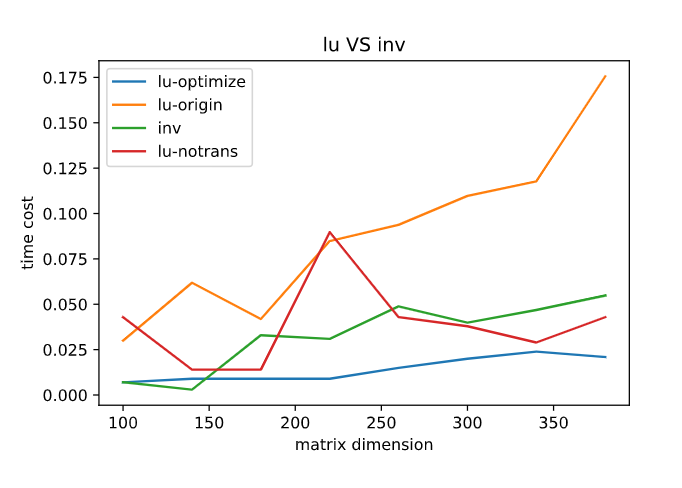
\includegraphics[width=180pt]{figures/comparison.png}
	\caption{通过LU求解线性方程组与通过求逆求解的效率比较}
	\label{fig:LU}
\end{figure}

\paragraph*{优化方法}
\\
\begin{itemize}
    \item 利用矩阵并行运算性质,将并行运算同步实现,将时间复杂度由$O(n^2)$降低到$O(n)$, 提高backward/forward substitution的效率
     \begin{figure}[ht]
        \centering
    	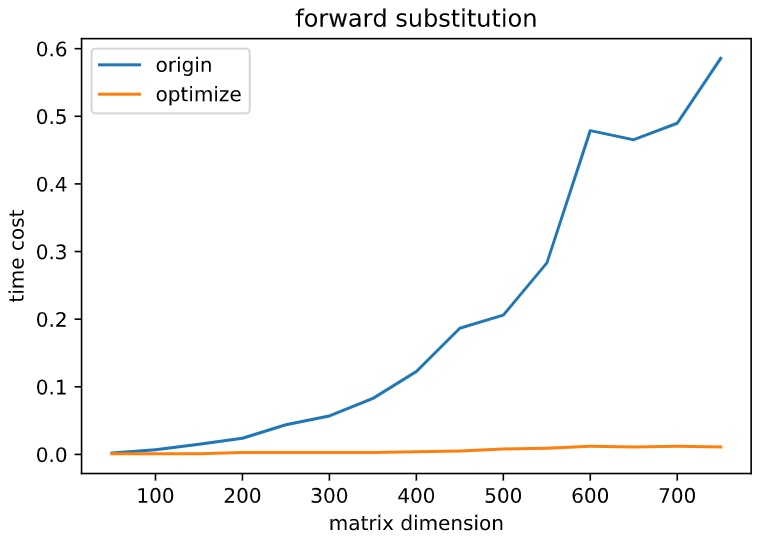
\includegraphics[width=180pt]{figures/forward_sub.png}
    	\caption{通过LU求解线性方程组与通过求逆求解的效率比较}
    	\label{fig:forward}
    \end{figure}
    \item 利用LU(PLU)中置换矩阵P的性质,有$P^{-1}=P^{T}$ 将求逆运算转换为求转置
\end{itemize}


\section{QR用于求特征值}
实数(分别是复数)非奇异矩阵A具有分解QR,其中Q正交,R所有元素为正。 这种因式分解是独特的,并且由Gram-Schmidt正交化过程给出(参见正交化方法)。 经常使用的特征值问题的QR算法(参见迭代方法)基于重复的QR分解。\cite{QR_wiki}

令 $A$ 我们想要计算特征根的实矩阵, 且 $A_{0}:=A$. 在第 $k$ 步 (从 $k=0$ 起始), 我们用 $\mathrm{QR}$ 分解计算 $A_{k}=Q_{k} R_{k}$,  其中$Q_{k}$ 是正交矩阵 (即, $Q^{T}=$ $\left.Q^{-1}\right)$ 且 $R_{k}$ 为上三角矩阵. 我们令 $A_{k+1}=R_{k} Q_{k}$.注意到有
$$
A_{k+1}=R_{k} Q_{k}=Q_{k}^{-1} Q_{k} R_{k} Q_{k}=Q_{k}^{-1} A_{k} Q_{k}=Q_{k}^{\top} A_{k} Q_{k}
$$
因此所有的 $A_{k}$ 具有相同的特征根. 这个算法是数值稳定的因为它是基于正交相似变换进行的。
\subsection{实现与优化}

核心步骤是两个算法:Gram-Schmidt正交化求出QR分解矩阵与QR算法求特征根
\paragraph{优化方法}
发现最初独立实现的QR效率远低于numpy的内置函数,通过分析,发现 Gram–Schmidt 的效率与行列向量数目相关,见图 \ref{fig:gram}
     \begin{figure}[ht]
        \centering
    	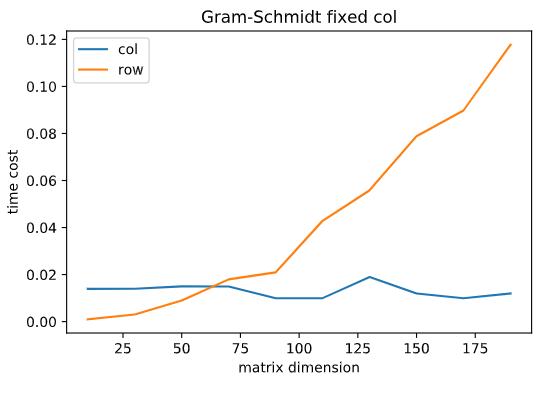
\includegraphics[width=180pt]{figures/gram_schmidt.png}
    	\caption{固定效率比较}
    	\label{fig:gram}
    \end{figure}
在对Gram-Schmidt算法进行优化后,并利用矩阵并行运算,得到的优化结果如下图\ref{fig:QR} 所示:
     \begin{figure}[ht]
        \centering
    	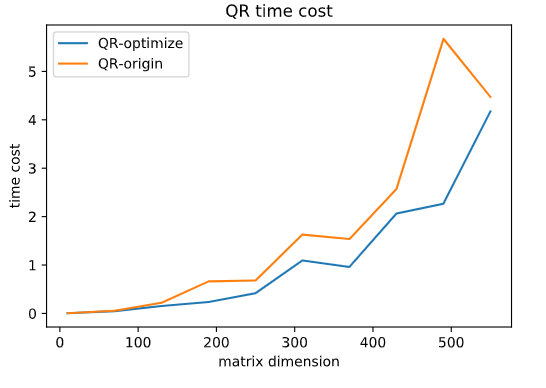
\includegraphics[width=180pt]{figures/QR.png}
    	\caption{优化前后QR分解效率比较}
    	\label{fig:QR}
    \end{figure}
\section{SVD用于图像压缩与推荐系统}
奇异值分解 $(\mathrm{SVD})$ 的传统应用是主成分分析 $(\mathrm{PCA})$ 。考虑推荐电影的问题。有 $n$ 个顾客, $d$ 个电影 矩阵 $A$ 的元素 $a_{i j}$ 表示顾客 $i$ 对电影 $j$ 的喜爱程度。假定有 $k$ 个决定顾客对电影的喜欢程度的基本因素,并咀 $k$ 远小于 $d$ 和 $n$ 。比如, 这些因素可以包括:喜剧、戏剧性、动作、新奇性的多少。每个电影可以通过一个 $k$ 维矢量来描述其包含的每个因子的多少,而每个顾客可以通过一个 $k$ 维矢量来描述其心目中不同因子的重 要性,这两个矢量的点乘就表示一个顾客对一个电影的喜爱程度。也就是说, $n \times d$ 的矩阵 $A$ 可以表示为 描述顾客的 $n \times k$ 矩阵 $U$ 与描述电影的 $k \times d$ 矩阵 $V$ 的乘积。通过SVD找出最佳的 $k$ 秩近似 $A_{k}$ 给出 $U$ 和 $V_{\text { }}$ $A$ 未必会精确等于 $U V$, 这种情况下 $A-U V$ 被当成噪声。另一个问题是, $\mathrm{SVD}$ 会给出包含负数的矩阵。 非负矩阵分解 (NMF ) 在某些情况下是更恰当的选择。
在上面的描述中, $A$ 是可完整获得的,我们希望通过 $U$ 和 $V$ 来找出基础矢量。但在现实情形, 比如在电影 推荐的情形, 每个顾客可能只看了少量电影, 也就是说更自然的假设是我们只知道 $A$ 的一部分元素, 然后 希望估计完整的 $A_{\circ}$ 如果 $A$ 是个一般的 $n \times d$ 矩阵, 则包含的信息量是 $\Omega(n d)$ 的量级, 因此不可能用很少 的数来估计。如果假定 $A$ 是一个低秩矩阵叠加上了一部分噪音,并且其元素是从某个分布随机取样的, 则 有可能可以用SVD来估计 $A$ 的总体。这被称为协同过滤, 这被用于推荐系统。\cite{SVD_PCA}

\subsection{图像压缩}

\subsubsection{原理}
使用SVD分解图片信息矩阵,保留一部分奇异值然后重构对角矩阵,达到简单的图片降噪和压缩的目的。
\subsubsection{效果}

1.原始图片  
\begin{figure}[h]
	\centering
	
\includegraphics[width=120pt]{figures/boy.jpeg}
	\caption{原始图像}
	\label{fig:1}
\end{figure}

2.压缩结果


\begin{figure}[h]
\centering
\begin{subfigure}{.5\textwidth}
	\centering
	
\includegraphics[width=120pt]{figures/boy30.jpg}
	\caption{保留30\%奇异值结果}
	\label{fig:boy3}
\end{subfigure}%
\begin{subfigure}{.5\textwidth}
    \centering
	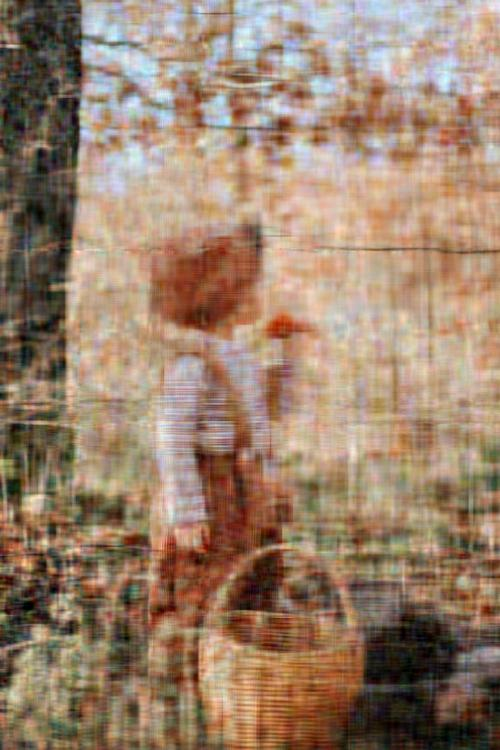
\includegraphics[width=120pt]{figures/boy50.jpg}
	\caption{保留50\%奇异值结果}
	\label{fig:boy5}
\end{subfigure}\\
\begin{subfigure}{.5\textwidth}
	\centering
	
\includegraphics[width=120pt]{figures/boy70.jpg}
	\caption{保留70\%奇异值结果}
	\label{fig:boy7}
\end{subfigure}%
\begin{subfigure}{.5\textwidth}
	\centering
	
\includegraphics[width=120pt]{figures/boy90.jpg}
	\caption{保留90\%奇异值结果}
	\label{fig:boy9}
\end{subfigure}
\caption{保留不同比例奇异值结果}
\label{fig:test}
\end{figure}


\subsubsection{总结}
保留的奇异值越多,图片的特征保留的越明显,当奇异值减少时,图片中的像素间的差距逐渐减小。
\subsection{推荐系统}

这里主要是应用在Netflix Prize中 大放异彩的 Funk SVD 算法,解决电影评分问题\cite{SVD_funk}


\subsubsection{传统 SVD 分解在元素缺失上面的问题}

历史上对缺失值的研究有很多,对于一个没有被打分的物品来说,到底是应该给它补一个 0 值,还是应该给它补一个平均值呢?由于在实际过程中,元素缺失值是非常多的,这就导致了早期的 SVD 不论通过以上哪种方法进行补全在实际的应用之中都是不可以被接受的。



\subsubsection{LFM (Latent Factor Model)}

直到 2006年 Netflix Prize 中 Simon Funk 在博客公开的算法。将评分矩阵分解成两个低维矩阵相乘,Simon Funk的思想很简单:可以直接通过训练集中的观察值利用最小化均方根学习P,Q矩阵。这种模型也被称作是 LFM (隐语义模型),下面是他当年的博客,有兴趣可以了解一下。


简单的来说就是将原本的 SVD 的思想上加上了线性回归,也就是说,我们可以用均方差作为损失函数,来寻找 P 和 q 的最终值,线性回归和均方差对于机器学习的同学们来说一定不陌生了,如果你还没有了解过,可能一下子理解不了下面的公式,那么我建议还是先从线性回归学起,便于理解。不过,线性回归也就是一句话 —— 线性函数参数调优。
\subsubsection{加入偏移项后的 Funk-SVD}

在 Funk-SVD 获得巨大成功之后,很多著名的模型都是对 Funk-SVD 进行缝缝补补得到的(详情可参见 Netflix Prize `Koren:2009` `Ricci:2010`),于是就有了在预测模型中添加三项偏移的模型,被称为 BaisSVD。
\begin{itemize}
    \item Biased Item(物品偏移),表示了物品接受的评分和用户没有多大关系,物品本身质量决定了的偏移。
    \item Biased User(用户偏移),有些用户喜欢打高分,有些用户喜欢打低分,用户决定的偏移。
    \item Biased Mean(全局平均值偏移),根据网站全局打分设置的偏移,可能和整体用户群和物品质量有相对应的关系。
\end{itemize}

\subsubsection{公式说明}
\paragraph{符号含义:}


\begin{itemize}
\centering
    \item $\gamma$ rates 学习率
    \item $\lambda$ regularization 正则化项
    \item $b$ biased 偏移
\end{itemize}





矩阵 M 经过Funk SVD 分解之后,只分解出两个矩阵P和Q:
$M_{m * n}=P_{m}^{T} * k Q_{k * n}$
对于某一个用户的评分使用 Funk SVD 进行矩阵分解得到的结果就是:
$$
\hat{r}_{u i}=\mu+b_{u}+b_{i}+q_{i}^{T} p_{u}
$$
那么我们需要最小化的损失函数就是:
$\sum_{r_{u i} \in R_{\text {train }}}\left(r_{u i}-\hat{r}_{u i}\right)^{2}+\lambda\left(b_{i}^{2}+b_{u}^{2}+\left\|q_{i}\right\|^{2}+\left\|p_{u}\right\|^{2}\right)$
损失就是:
$e_{u i}=r_{u i}-\hat{r}_{u i}$
使用随机梯度下降调参:
$$
\begin{array}{c}
b_{u} \leftarrow-b_{u}+\gamma\left(e_{u i}-\lambda b_{u}\right. \\
b_{i}<-b_{i}+\gamma\left(e_{u i}-\lambda b_{i}\right) \\
p_{u} \leftarrow p_{u}+\gamma\left(e_{u i} \cdot q_{i}-\lambda p_{u}\right) \\
q_{i}<-q_{i}+\gamma\left(e_{u i} \cdot p_{u}-\lambda q_{i}\right)
\end{array}
$$
还有一种情况就是,抛弃biased, 也就是:
$\hat{r}_{u i}=q_{i}^{T} p_{u}$
\subsubsection{结果}
在利用Funk SVD算法进行预测后,部分结果如下:
     \begin{figure}[ht]
        \centering
    	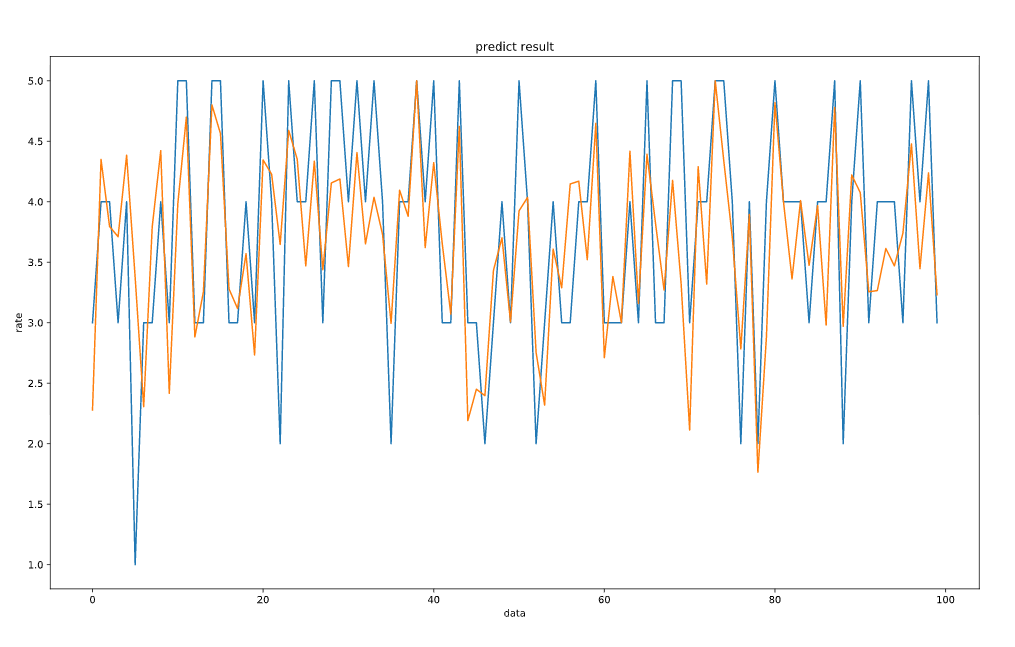
\includegraphics[width=\textwidth]{figures/recommend.png}
    	\caption{预测与真实值的对比}
    	\label{fig:Funk_SVD}
    \end{figure}

%此处结束正文-------------------------------------------------------------------------------------------------
%%%============================================================================================================%%%

%%%=== 参考文献 ========%%%
\cleardoublepage\phantomsection
\addcontentsline{toc}{chapter}{参考文献}
\renewcommand{\baselinestretch}{1.6}
\begin{thebibliography}{00}

  \bibitem{matrix_wiki} matrix decomposition.  \url{https://en.wikipedia.org/wiki/Matrix_decomposition}.
  
  \bibitem{matrix_jiqi} 矩阵分解.  \url{https://www.jiqizhixin.com/graph/technologies/775b8e6a-d0e4-42cd-a837-d587e4181470}.
  
  \bibitem{gram} Gram–Schmidt process, \url{https://en.wikipedia.org/w/index.php?title=Gram%E2%80%93Schmidt_process&oldid=1013879869} (last visited May 12, 2021)

  \bibitem{QR_wiki}   QR algorithm, \url{https://en.wikipedia.org/w/index.php?title=QR_algorithm&oldid=995579135} (last visited May 12, 2021).
  
  \bibitem{SVD} 刘建平Pinard. 奇异值分解(SVD)原理与在降维中的应用. \url{https://www.cnblogs.com/pinard/p/6251584.html}
  
  \bibitem{SVD_PCA}Hopcroft 《数据科学基础》第四章:奇异值分解\url{http://fjdu.github.io/data/science/2016/05/06/hopcroft-chap-4.html}
    \bibitem{SVD_funk}Hopcroft 推荐算法入门(2)SVD 和 Netflix Prize 的 Funk-SVD 篇\url{https://zhuanlan.zhihu.com/p/33262521}
  

\end{thebibliography}

\cleardoublepage
\end{document}
